%  Document Config
\documentclass[12pt]{diazessay}
\title{\textbf{CSC361: Bridge And Flashlight Problem} \\ {\Large\itshape King Saud University}}

\author{\textbf{Authors} \\ \textit{Mohand Al-Rasheed,\\}\textit{Name1,\\}\textit{Will edit this later to add ksu logo, names \& numbers project supiverser, logo, name, subject details }} 

% Image config
\usepackage{graphicx}
\graphicspath{ {./Figures/} }

% Code config
\usepackage{listings}
\usepackage{color}

\definecolor{dkgreen}{rgb}{0,0.6,0}
\definecolor{gray}{rgb}{0.5,0.5,0.5}
\definecolor{mauve}{rgb}{0.58,0,0.82}
\definecolor{backcolour}{rgb}{0.99,0.99,0.99}


\lstset{frame=tb,
  language=Python,
  aboveskip=3mm,
  belowskip=3mm,
  showstringspaces=false,
  columns=flexible,
  basicstyle={\small\ttfamily},
  backgroundcolor=\color{backcolour},   
  numbers=left,
  numberstyle=\tiny\color{gray},
  keywordstyle=\color{blue},
  commentstyle=\color{dkgreen},
  stringstyle=\color{mauve},
  breaklines=True,
  breakatwhitespace=true,
  tabsize=1
}


% Section config
\usepackage{titlesec}
\usepackage{hyperref}

\titleclass{\subsubsubsection}{straight}[\subsection]

\newcounter{subsubsubsection}[subsubsection]
\renewcommand\thesubsubsubsection{\thesubsubsection.\arabic{subsubsubsection}}
\renewcommand\theparagraph{\thesubsubsubsection.\arabic{paragraph}} % optional; useful if paragraphs are to be numbered

\titleformat{\subsubsubsection}
  {\normalfont\normalsize\bfseries}{\thesubsubsubsection}{1em}{}
\titlespacing*{\subsubsubsection}
{0pt}{3.25ex plus 1ex minus .2ex}{1.5ex plus .2ex}

\makeatletter
\renewcommand\paragraph{\@startsection{paragraph}{5}{\z@}%
  {3.25ex \@plus1ex \@minus.2ex}%
  {-1em}%
  {\normalfont\normalsize\bfseries}}
\renewcommand\subparagraph{\@startsection{subparagraph}{6}{\parindent}%
  {3.25ex \@plus1ex \@minus .2ex}%
  {-1em}%
  {\normalfont\normalsize\bfseries}}
\def\toclevel@subsubsubsection{4}
\def\toclevel@paragraph{5}
\def\toclevel@paragraph{6}
\def\l@subsubsubsection{\@dottedtocline{4}{7em}{4em}}
\def\l@paragraph{\@dottedtocline{5}{10em}{5em}}
\def\l@subparagraph{\@dottedtocline{6}{14em}{6em}}
\makeatother

\setcounter{secnumdepth}{4}
\setcounter{tocdepth}{4}





\date{} 
\begin{document}


\maketitle % Print the title section
\clearpage

%----------------------------------------------------------------------------------------
%	ESSAY BODY
%----------------------------------------------------------------------------------------

\tableofcontents

\cleardoublepage

\addcontentsline{toc}{section}{Acknowledgements}
\section*{Acknowledgements}

\addcontentsline{toc}{section}{English Abstract}
\section*{English Abstract}

\addcontentsline{toc}{section}{Arabic Abstract}
\section*{Arabic Abstract}

\section{Introduction}

    \subsection{Problem statement}
    
    Dialects are formed and differ due to a main factor. It is the isolation between the environments of the Arab community. The isolation is due to the different social conditions within a single language community. This solitude separated Arab people, and reduces the friction between them. And as a result of that, many Arabic speaking regions have formed dialects exclusive to their own. For example, many countries surrounding the Arabic Gulf have formed a dialect different to countries in the Levantine region. So, the research’s main problem is how to identify and predict the dialect in the written text.

 
    \begin{figure}[h]
        % \hskip-3.3cm
        \centering
        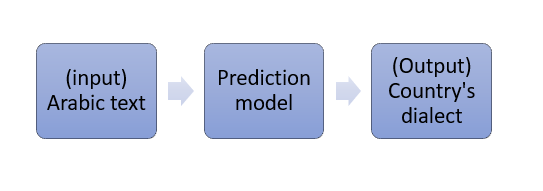
\includegraphics[scale=0.6]{Figures/problem_statment_fig.png}
        \caption{Illustration of the problem}
        \label{fig:cmp}
    \end{figure}
        
    % Figure 1.1: Illustration of the problem

    
    \subsection{Goals and objectives}
    
    The goal of this research is to analyze an Arabic text to extract the dialect of the given text.
    The objective is to collect text from many different dialects, and implement the most appropriate state of the art model in NLP that helps in achieving the best possible accuracy and provides from which dialect the text is .

    \subsection{Proposed Solution}
    
    This research will contribute in solving Arabic dialect detection by gathering more Arabic dialect text beside what we have, searching for the most appropriate dialect prediction approaches, and using one of the latest advanced model in NLP field.
    
    \subsection{Research scope}
    
    In this research we will gather more Arabic dialect text besides what we have, preprocess them, train the chosen model and use the model to predict any Arabic dialect text. 

\section{Background}

    \subsection{Natural language processing}
    
    \subsection{Preprocessing}

    \subsection{Dialect prediction approaches}
    
        \subsubsection{Approach 1}
        \subsubsection{Approach 2}
        \subsubsection{Approach 3}


% USE ANYTHING LOWER THAN THIS AS A QUICK GUIDE
\section{Representation}
    \subsection{State Representation}
        Given the problem structure, we can represent any one person being on the east or the west by a Boolean value, where \textit{False} represents the person being on the east and \textit{True} represents the person being on the west. The same logic can be applied to the flashlight position. We bundle all the positions of people in an array and include the flashlight position, this structure can fully represent the state at any given position.
        \paragraph{Initial State}
            The initial state for this problem is \textit{(False, False, ..), False)}
        \paragraph{Goal State}
            The goal state for this problem is \textit{(True, True, ..), True)}
        
        
    \subsection{Data Structures}
        In order for us to solve this problem using searching algorithms, we have to define specific data structures that allow us to traverse the state space efficiently, we create a \textit{Node} and a \textit{Problem} structures to house the state and problem inputs respectively. 
        \subsubsection{BridgeNode}
            In each node we store a couple of different values that are useful to us
            \begin{enumerate}
                \item State
                \item Parent Node
                \item Depth
                \item Path Cost
            \end{enumerate}
            We also define the comparison operators between nodes to compare the path cost of each node
        \subsubsection{BridgeProblem}
            In the problem structure we store the inputs of the problem as well as the initial node and also several valuable functions.
            \paragraph{Successor function}
                By expanding a node we return nodes that success it, for example given the initial node with state \textit{[False, False], False}, states that success it are:
                \begin{enumerate}
                    \item \textit{[True, False], True}
                    \item \textit{[False, True], True}
                    \item \textit{[True, True], True}
                \end{enumerate}
                An algorithm for finding successor states can be formulated as follows:
                \begin{lstlisting}
                    # Input: State
                    # Output: List of States
                    m <- min_num_ppl_crossing
                    n <- max_num_ppl_crossing
            
                    positions, flash_is_west <- start_state
                    result <- []
                    legal_positions <- []
            
                    for i in 0..length(positions)-1:
                        if positions[i] = flash_is_west:
                            legal_positions.add(i)
            
                    for comb_indices in combinations(legal_positions, r) for r in m..n:
                        newPositions <- newPositions
                        for index in comb_indices:
                            newPositions[index] <- !newPositions[index]
                        result.add(State((newPositions, not flash_is_west)))
                    return result
                \end{lstlisting}
                By modifying \textit{m} and \textit{n} we can generalize the problem such that the minimum number of people moving each turn isn't 1 but \textit{m}, the same thing for the maximum number of people moving each turn.

            \paragraph{Goal Test}
                We have to check weather a node is the goal state or not. Checking for goal state involves checking that every person made it to the left of west, i.e. every position in the node's state is True. Here's the algorithm for goal test
                \begin{lstlisting}
                    positions <- node.state[0] # Positions
                    for position in positions:
                        if position is False:
                            return False
                    return True
                \end{lstlisting}
        \subsubsection{Additional Data Structures}
            We used \textit{Priority Heaps} to organize our search based on the priority of any given node (more on that in the Algorithms section). We also used structures to keep \& count all the evaluation data (e.g. \textit{Solution Cost}, etc.).
    
    \subsection{Repeated States}
        By expanding any given node all the nodes inside can be expanded to return to the original node, which can turn a linear problem to an exponential one. We use this fact to optimize some of our algorithms and compare the running time of each later.

\section{Algorithms}{
    In each of the following algorithms we used the implementation detailed in \textit{A Modern Approach, Acting rationally}\cite{Artificial Intelligence: A Modern Approach}.
    \paragraph{Uniform Cost Search}
        Uniform Cost Search (abbreviated UCS) is a node expansion strategy that expands the nodes with the least cost, we used a \textit{Priority Heap} data structure in organizing the nodes in the queue, where the priority is gotten from the \textit{path cost} in the node's data.
    \paragraph{Iterative Deepening Search}
        Iterative Deepening Search (abbreviated IDS) is a depth first search variant that expands nodes starting from $Depth = 1$ until $Depth = \infty$ recursively, which saves up memory cost immensely.
    \paragraph{A* Search}
        A* Search or A* uses the \textit{path cost} as well as a value $h(node.state)$ which allows it predict the node with the most potential. We arrived at a heuristic function \textit{h} by relaxing the flashlight constraint then calculated the cost. This allows for an admissible heuristic. \\
        The function approximates the remaining cost by taking the minimum cost possible on the east side of the bridge. This ensures optimally of the result\cite{Artificial Intelligence: A Modern Approach}. \\
        Here's the algorithm
        \begin{lstlisting}
            # Input: State, problem
            # Output: Integer (Cost)
            costs <- []
            for index in 0..length(state.positions)-1:
                if !state.positions[index]:
                    costs.add(problem.cost_arr[index])
                    
            if length(costs) = 0:
                return 0
    
            costs = sort_ascending(costs)
            if length(costs) % 2 != 0:
                costs.append(0)
            cost = 0
            
            for chunk in chunks_of_two(costs):
                cost += chunk[0]
                
            return cost
        \end{lstlisting}
}


\clearpage
\section{Results}    
    \subsection{Performance}
        We calculated the performance of each algorithm on three dimensions
        \begin{enumerate}
            \item \textit{Solution Cost}: The number of nodes in the solution
            \item \textit{Search Cost}: The number of nodes generated during search
            \item \textit{Space Requirement}: The number of nodes concurrently in the priority queue during search
        \end{enumerate}
        We then optimized UCS, IDS and A* to ignore repeated states since they make no difference in the search and take a lot of unnecessary time and memory.
        \subsubsection{Performance}
\begin{tabular}{lllll}
\toprule
            &                            &        UCS &        IDS &         A* \\
Test Case & Metric &            &            &            \\
\midrule
( 1 2 ) & Solution Cost &          2 &          2 &          2 \\
            & Search Cost &          1 &          3 &          1 \\
            & Space Requirement &          1 &          2 &          1 \\
            & Time (s) &   3.82e-05 &   3.49e-05 &   4.71e-05 \\
( 3 2 5 ) & Solution Cost &         10 &         11 &         10 \\
            & Search Cost &         15 &         22 &         14 \\
            & Space Requirement &          4 &          4 &          4 \\
            & Time (s) &  0.0001595 &   0.000154 &  0.0001857 \\
( 1 3 2 5 ) & Solution Cost &         12 &         12 &         12 \\
            & Search Cost &         66 &        122 &         63 \\
            & Space Requirement &          9 &          6 &          8 \\
            & Time (s) &  0.0004984 &  0.0007511 &  0.0007958 \\
( 1 9 2 1 ) & Solution Cost &         13 &         14 &         13 \\
            & Search Cost &         66 &        122 &         61 \\
            & Space Requirement &          9 &          6 &          9 \\
            & Time (s) &  0.0005281 &  0.0008551 &  0.0006944 \\
( 3 3 3 3 ) & Solution Cost &         15 &         15 &         15 \\
            & Search Cost &         66 &        122 &         66 \\
            & Space Requirement &          7 &          6 &          7 \\
            & Time (s) &  0.0005001 &  0.0007254 &  0.0008629 \\
\bottomrule
\end{tabular}

\vspace{10pt}
        \subsubsection{Solutions}
\vspace{10pt}










\subsubsubsection{UCS} 
\begin{tabular}{llllll}
\toprule
{} &      ( 1 2 ) &    ( 3 2 5 ) &  ( 1 3 2 5 ) &  ( 1 9 2 1 ) &  ( 3 3 3 3 ) \\
\midrule
0  &  Move a0, a1 &  Move a0, a1 &  Move a0, a2 &  Move a0, a3 &  Move a0, a2 \\
1  &              &    Return a1 &    Return a0 &    Return a3 &    Return a2 \\
2  &              &  Move a1, a2 &  Move a0, a1 &  Move a1, a2 &  Move a1, a2 \\
3  &              &              &    Return a0 &    Return a0 &    Return a1 \\
4  &              &              &  Move a0, a3 &  Move a0, a3 &  Move a1, a3 \\
\bottomrule
\end{tabular}

\vspace{1cm}

\subsubsubsection{IDS}
\begin{tabular}{llllll}
\toprule
{} &      ( 1 2 ) &    ( 3 2 5 ) &  ( 1 3 2 5 ) &  ( 1 9 2 1 ) &  ( 3 3 3 3 ) \\
\midrule
0  &  Move a0, a1 &  Move a0, a1 &  Move a0, a1 &  Move a0, a1 &  Move a0, a1 \\
1  &              &    Return a0 &    Return a0 &    Return a0 &    Return a0 \\
2  &              &  Move a0, a2 &  Move a0, a2 &  Move a0, a2 &  Move a0, a2 \\
3  &              &              &    Return a0 &    Return a0 &    Return a0 \\
4  &              &              &  Move a0, a3 &  Move a0, a3 &  Move a0, a3 \\
\bottomrule
\end{tabular}

\vspace{1cm}

\subsubsubsection{A*}
\begin{tabular}{llllll}
\toprule
{} &      ( 1 2 ) &    ( 3 2 5 ) &  ( 1 3 2 5 ) &  ( 1 9 2 1 ) &  ( 3 3 3 3 ) \\
\midrule
0  &  Move a0, a1 &  Move a0, a1 &  Move a0, a2 &  Move a0, a3 &  Move a0, a2 \\
1  &              &    Return a1 &    Return a0 &    Return a0 &    Return a2 \\
2  &              &  Move a1, a2 &  Move a0, a1 &  Move a1, a2 &  Move a1, a2 \\
3  &              &              &    Return a0 &    Return a3 &    Return a1 \\
4  &              &              &  Move a0, a3 &  Move a0, a3 &  Move a1, a3 \\
\bottomrule
\end{tabular}



    \subsection{Additional Test Cases}
\hskip-2.8cm
\begin{tabular}{lllll}
\toprule
                        &                            &        UCS &        IDS &         A* \\
Test Case & Metric &            &            &            \\
\midrule
( 9 9 9 9 9 9 30 ) & Solution Cost &        120 &        120 &        120 \\
                        & Search Cost &       1757 &       3772 &       1757 \\
                        & Space Requirement &         62 &         12 &         52 \\
                        & Time (s) &  0.0328977 &  0.0215698 &  0.0320076 \\
( 44 55 66 33 8 1 ) & Solution Cost &        152 &        429 &        152 \\
                        & Search Cost &        640 &       1398 &        345 \\
                        & Space Requirement &         41 &         10 &         64 \\
                        & Time (s) &  0.0088175 &  0.0077256 &   0.008262 \\
( 5 6 4 3 3 4 5 6000 ) & Solution Cost &       6039 &       6061 &       6039 \\
                        & Search Cost &       4564 &       9359 &       4519 \\
                        & Space Requirement &        146 &         14 &        125 \\
                        & Time (s) &   0.145964 &  0.0540114 &   0.165986 \\
( 50 60 40 30 30 40 50 6 ) & Solution Cost &        336 &        660 &        336 \\
                        & Search Cost &       4564 &       9359 &       4456 \\
                        & Space Requirement &        116 &         14 &        136 \\
                        & Time (s) &   0.146448 &  0.0553102 &    0.17063 \\
( 10 100 1000 10000 1000 100 10 1 ) & Solution Cost &      11164 &      12280 &      11164 \\
                        & Search Cost &       4564 &       9359 &       4458 \\
                        & Space Requirement &        186 &         14 &        129 \\
                        & Time (s) &   0.150916 &  0.0546698 &   0.175499 \\
( 100 2 3 4 5 60 7 8 9 ) & Solution Cost &        149 &       1500 &        149 \\
                        & Search Cost &      11465 &      22875 &       5780 \\
                        & Space Requirement &        381 &         16 &        560 \\
                        & Time (s) &   0.710664 &    0.13129 &   0.764477 \\
( 3 3 3 4 4 4 4 8 8 ) & Solution Cost &         52 &         59 &         52 \\
                        & Search Cost &      11465 &      22875 &      11235 \\
                        & Space Requirement &        230 &         16 &        325 \\
                        & Time (s) &   0.703197 &   0.131648 &   0.838294 \\
( 10 20 30 40 50 60 70 80 90 100 ) & Solution Cost &        500 &        620 &        500 \\
                        & Search Cost &      28093 &      51812 &      27511 \\
                        & Space Requirement &        472 &         18 &        529 \\
                        & Time (s) &    3.22846 &   0.343196 &    4.01714 \\
( 100 90 80 70 60 60 70 80 90 100 ) & Solution Cost &       1120 &       1700 &       1120 \\
                        & Search Cost &      28095 &      51812 &      28045 \\
                        & Space Requirement &        346 &         18 &        503 \\
                        & Time (s) &    2.61024 &   0.303756 &    3.23587 \\
( 5 5 5 5 5 5 5 5 5 5 ) & Solution Cost &         85 &         85 &         85 \\
                        & Search Cost &      28095 &      51812 &      28095 \\
                        & Space Requirement &        368 &         18 &        368 \\
                        & Time (s) &    2.29129 &   0.304314 &    2.29675 \\
\bottomrule
\end{tabular}


        \begin{figure}[h]
            \hskip-3.3cm
            \includegraphics[scale=0.3]{Figures/AlgoCompr.png}
            \caption{Plot additional Test Cases}
            \label{fig:cmp}
        \end{figure}

    \subsection{Visualizations}
        Here we will visualize some of the different subsets of the state space. 
        The label of any node is two parts, the number before the underscore signifies when the algorithm generated this node and what's after the underscore is a compact representation of the state at the current node, such that 0 at the ith index means the $a_0$ is at the east, and a 1 at the ith index means  $a_i$ is at the west.
        \subsubsection{Solution Tree Visualization}
            We can visualize a subset of the state space for us to have a better idea of what the algorithm is trying.
            Here is a visualization of all nodes visited by each algorithm.
                \paragraph{UCS} The test case visualized is  \textit{(3 2 5)}
                \hskip-4.0cm
                \begin{figure}[h]
                    \centering
                    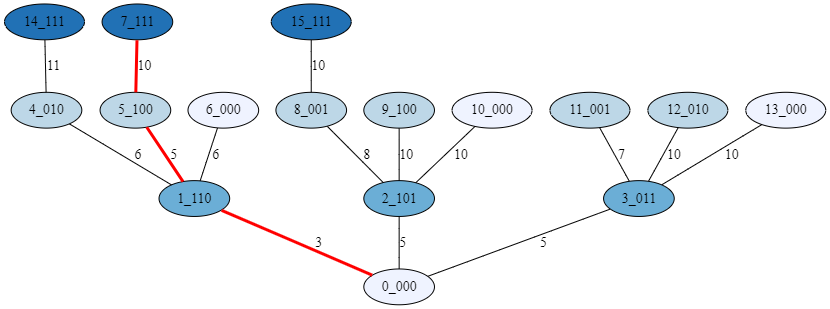
\includegraphics[width=\textwidth]{Figures/UCS optimized.png}
                    \caption{Uniform Cost Search expands the least cost node}
                    \label{fig:UCS}
                \end{figure}
                
                \clearpage
                \paragraph{IDS} The test case visualized is  \textit{(3 2 5)}
                \hskip-4.0cm
                \begin{figure}[h]
                    \centering
                    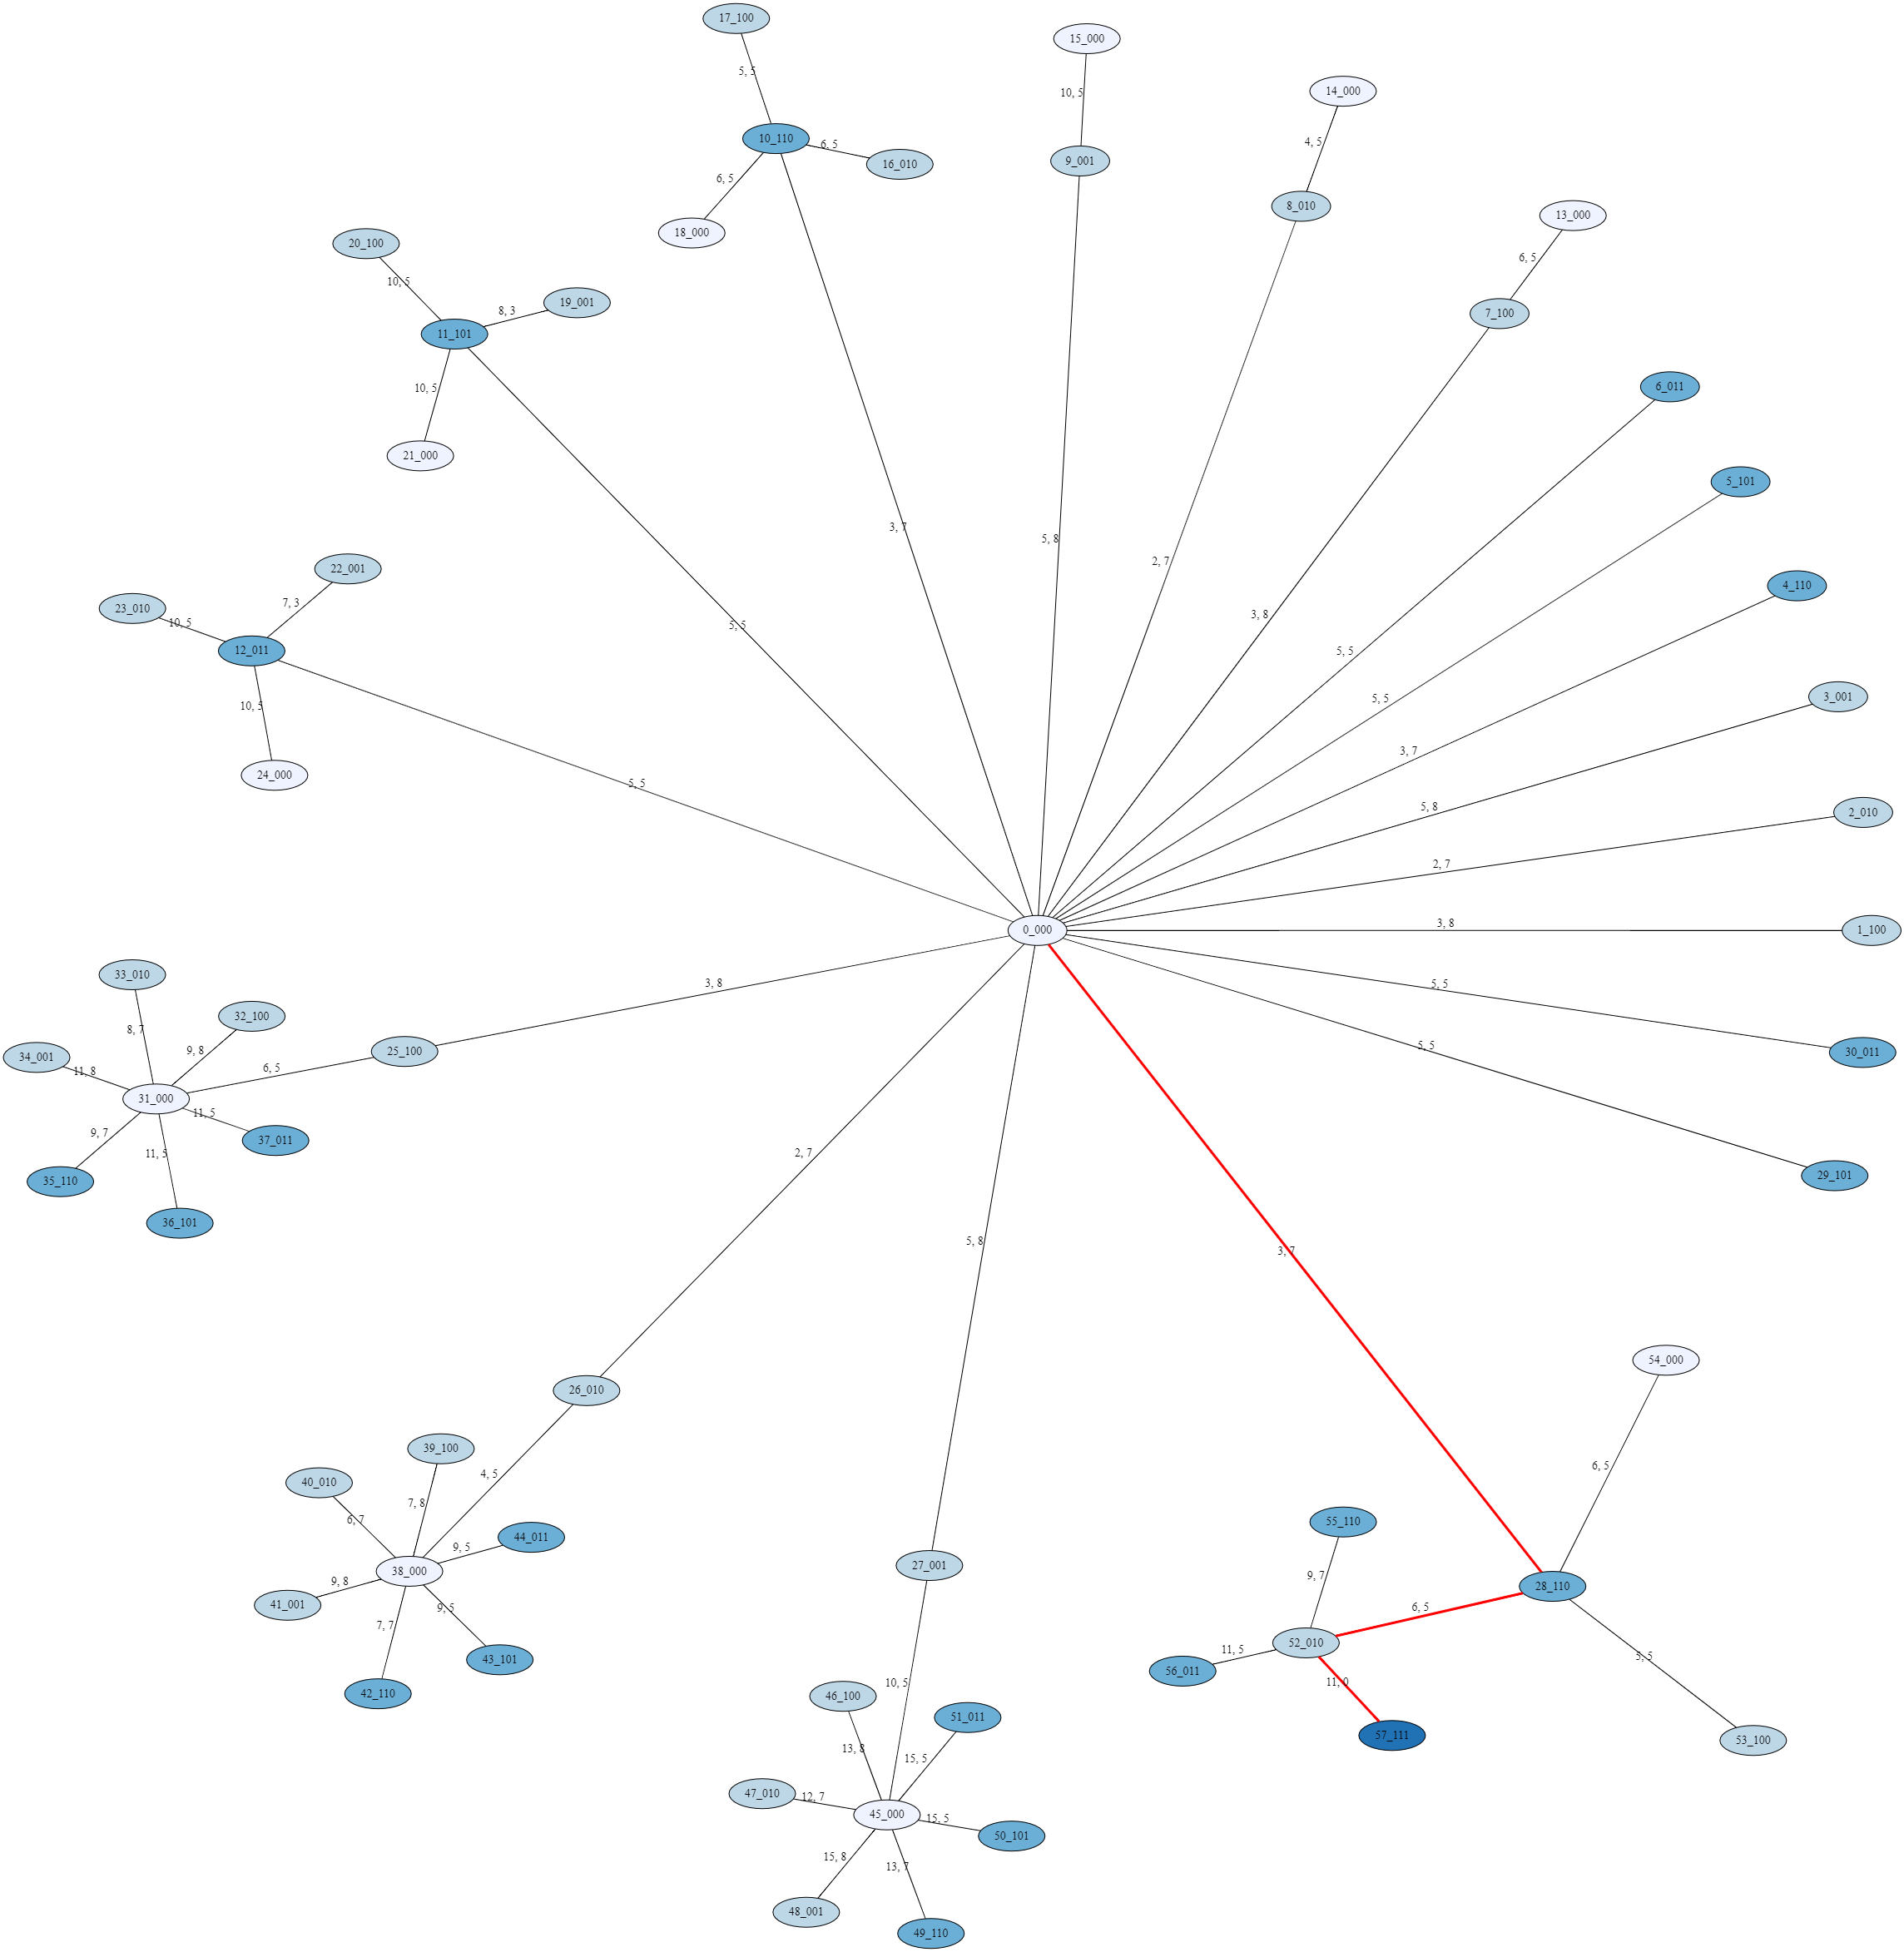
\includegraphics[width=\textwidth]{Figures/IDS.png}
                    \caption{Iterated Deepening Search recursively repeats searching to conserve memory}
                    \label{fig:IDS}
                \end{figure}
                
                \clearpage
                \paragraph{A*} The test case visualized is  \textit{(3 2 5)}
                \hskip-4.0cm
                \begin{figure}[h]
                    \centering
                    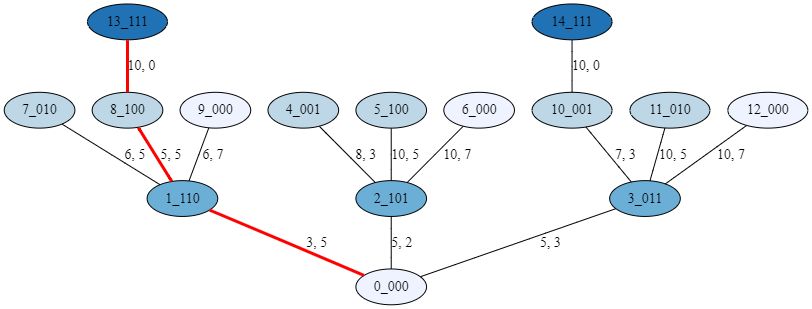
\includegraphics[width=\textwidth]{Figures/AStar.png}
                    \caption{A* Uses a heuristic to predict the real cost}
                    \label{fig:A*}
                \end{figure}
                \\
                we can see the left most node is not visited by A* even though UCS visits that node, the reason for that is that the predicted cost of visiting it heavily outweighs the cost of visiting other nodes.
                \clearpage
        \subsubsection{State Space Visualization}
            We can merge nodes with similar states to have a better idea of the problem the algorithms are traversing. 
            The test case visualized is  \textit{(2 3 2 5)}
            \hskip-4.0cm
            \begin{figure}[h]
                \centering
                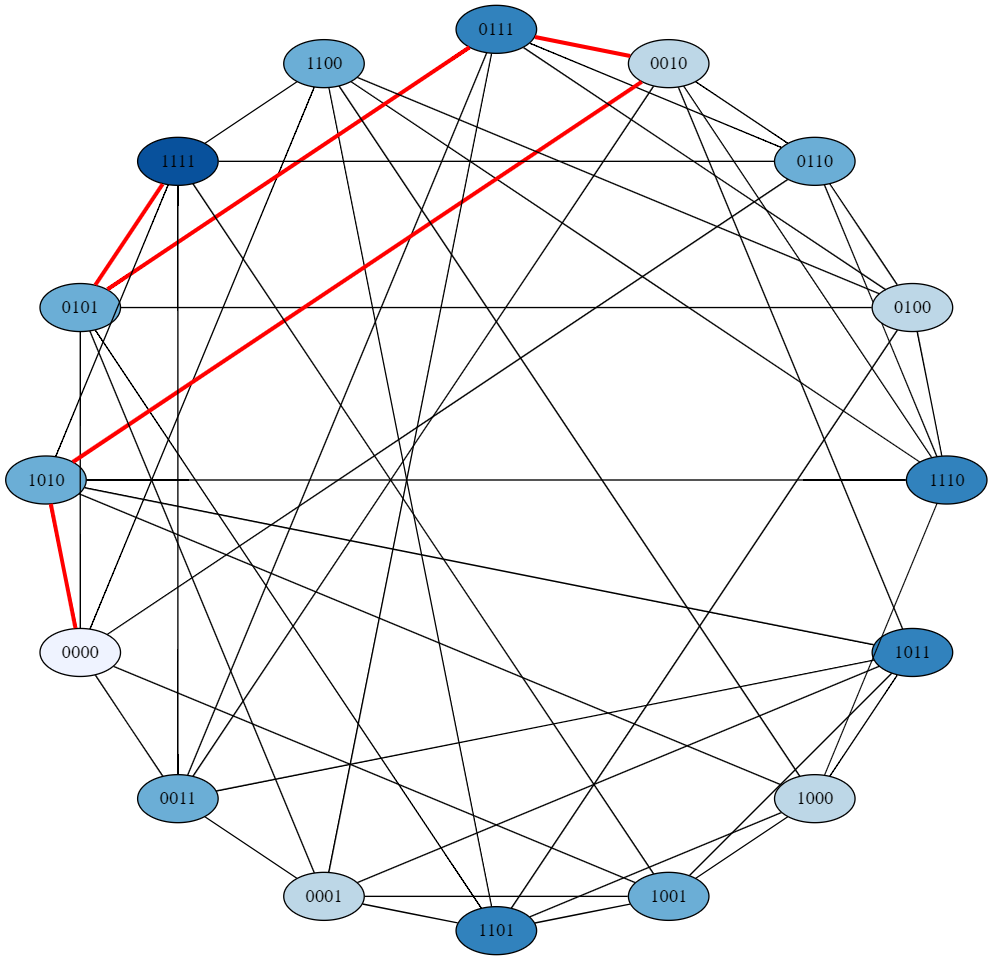
\includegraphics[width=\textwidth]{Figures/State space for k=4.png}
                \label{fig:A*}
            \end{figure}

\clearpage
\section{Conclusions \& Future work}
    Searching algorithms vary in their performance, we concluded that A* has the slow run-time (given our heuristic function), and Iterated Deepening Search has a low memory usage which is sometimes essential, though heavily lacking in speed. Optimizing for repeated states adds enormous amount of speedup to our algorithms.
    \subsection{Future Work}
        \paragraph{Generalized Bridge And Flashlight Problem} We can generalize the Bridge And Flashlight problem by changing the minimum number of people crossing the bridge \textit{m} or increasing the number of maximum number of people crossing \textit{n}, not all instances of this generalization are solvable, though some pose an interesting problem.
        \paragraph{Bidirectional Search} Given this problem's goal, we can run a bidirectional search that backtracks from the solution and also traverses the tree from the initial node, this can massively cut-down on the complexity growth.

\bibliographystyle{unsrt}
\begin{thebibliography}{9}

\bibitem{Artificial Intelligence: A Modern Approach} 
Artificial Intelligence: A Modern Approach,
\textit{Searching Strategies}. \\
Peter Norvig and Stuart J. Russell
% \\\texttt{https://people.eecs.berkeley.edu/~russell/intro.html}


% \bibitem{convertize} 
% Convertize
% \textit{The Scarcity Effect}. 
% \\\texttt{https://www.convertize.com/glossary/scarcity-effect/}
\end{thebibliography}

\end{document}
